\documentclass[oribibl]{llncs}

\usepackage{cite}
\usepackage{amsmath}
\usepackage{amsfonts}
\usepackage{graphicx}
\usepackage{url}
\usepackage{footmisc}
\usepackage{color}

\renewcommand{\Re}{\mathbb{R}}
\renewcommand{\thefootnote}{\fnsymbol{footnote}}

\begin{document}

\title{Improvements of a Fast Parallel Poisson Solver on Irregular
  Domains}

\frontmatter

\pagestyle{plain}
\pagenumbering{arabic}

\author{Andreas Adelmann\inst{1}
  \and
  Peter Arbenz\inst{2}\thanks{Corresponding author.
    Email: \texttt{arbenz@inf.ethz.ch}}
  \and
  Yves Ineichen\inst{1,2}
}

\institute{Paul Scherrer Institut, Villigen, Switzerland
  \and%
  ETH Z\"urch, Chair of Computational Science, Z\"urich, Switzerland
}

\maketitle

\begin{abstract}
  We discuss the scalable parallel solution of the Poisson equation on
  irregularly shaped domains discretized by finite differences.  The
  symmetric positive definite system is solved by the preconditioned
  conjugate gradient algorithm with smoothed aggregation (SA) based
  algebraic multigrid (AMG) preconditioning.  We investigate variants of
  the implementation of SA-AMG that lead to considerable improvements in
  the execution times.  The improvements are due to a better data
  partitioning and the iterative solution of the coarsest level system
  in AMG.  We demonstrate good scalability of the solver on a
  distributed memory parallel computer with up to 2048 processors.

\end{abstract}

\keywordname\ Poisson equation, finite differences, preconditioned
conjugate gradient algorithm, algebraic multigrid, data partitioning.

\section{Introduction}
\label{sec:intro}

The solver described in this paper is part of the general accelerator
modeling tool Object Oriented Parallel Accelerator Library
(OPAL)~\cite{opal}.  OPAL enables the solution of the most challenging
problems in the field of high precision particle accelerator modeling.
These include the simulation of high power hadron accelerators and of
next generation light sources.

In these simulations the evolution of the charged particles is
determined by the collisionless \emph{Vlasov equation}.  The most
compute intense portion of the simulation is the determination of the
electrostatic potential $\phi$ from the \emph{Poisson equation}
\begin{equation}\label{eq:poisson0}
  - \varepsilon_0\, \Delta {\phi}(\mathbf{x}) =
  {\rho}(\mathbf{x}),
\end{equation}
in a coordinate system moving with the particles.  Here, $\rho$ denotes
the spatial charge density and $\varepsilon_0$ is the dielectric
constant.  The electric field is obtained from
\begin{equation}\label{eq:e-field}
  \mathbf{E} = -\nabla{\phi}.
\end{equation}
An appropriate \emph{Lorentz transformation} yields the electromagnetic
fields in the static reference frame that are needed to move the
particles.  For details see~\cite{adai:10}.

The Poisson problem~\eqref{eq:poisson0} discretized by finite
differences can efficiently be solved on a rectangular grid by a
Particle-In-Cell (PIC) approach~\cite{qiry:01}.  The right hand side
in~\eqref{eq:poisson0} is discretized by sampling the particles at the
grid points.  In~\eqref{eq:e-field}, ${\phi}$ is interpolated at the
particle positions from its values at the grid points.  We also note
that the common FFT-based Poisson solvers and similar
approaches~\cite{qiry:01,qigl:04} are restricted to box-shaped or open
domains.

In section~\ref{sec:discr} we present our finite difference approach and
how we treat the boundary at curved surfaces.  In
section~\ref{sec:method} we review the iterative system solver.  In
section~\ref{sec:analysis} we discuss numerical experiments on 512--2048
processors of a Cray XT-5.  In particular, we are interested in the
partitioning of the computational domain and in the coarse level solver
of the multilevel preconditioner.  Section~\ref{sec:concl} concludes the
paper.

\section{The discretization}
\label{sec:discr}

In this section we discuss the solution of the Poisson equation in a
domain 
%%
\begin{figure}[htb]
  \centering
  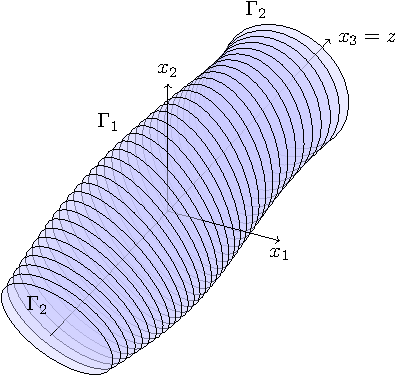
\includegraphics[width=0.35\textwidth]{figbound.pdf}
  \caption{Sketch of a typical domain}
  \label{fig:domain}
\end{figure}
%%
$\Omega \subset \Re^3$ as indicated in Fig.~\ref{fig:domain}.  The
boundary of the domain is composed of two parts, a curved, smooth
surface $\Gamma_1$ and two planar portions at $z=-d$ and $z=+d$ that
form together $\Gamma_2$.  In physical terms $\Gamma_1$ forms the casing
of the pipe, while $\Gamma_2$ is the open boundary at the inlet and
outlet of the beam pipe, respectively.  The centroid of the particle
bunch is at the origin of the coordinate system.  In practice the shape
of $\Gamma_1$ can be quite complicated.  Our code assumes that a ray
that emanates perpendicularly from the $z$-axis crosses $\Gamma_1$ at
most once.

The Poisson problem that we are going to solve is given by
\begin{equation} \label{eq:poisson}
  \begin{gathered}
    -\epsilon_0\, \Delta \phi = \rho\ \text{in}\ \Omega, \\
    \phi = g \equiv 0\ \text{on}\ \Gamma_1, \quad
    \partial_n{\phi} +  (1/d) \phi = 0\
    \text{on}\ \Gamma_2.
  \end{gathered}
\end{equation}
The parameter $d$ in the Robin boundary condition is half the extent of
$\Omega$ in $z$-direction~\cite{poplau_self-adaptive_2008}.

We discretize~\eqref{eq:poisson} by a standard second order finite
difference scheme defined on a rectangular grid with grid spacing $h_i$
in the $i$-th coordinate direction.  It is natural to arrange the grid
such that the two portions of $\Gamma_2$ lie in grid planes.

A lattice point is called an \emph{interior} point if all its direct
neighbors are in $\Omega$.  All other grid points are called
\emph{near-boundary} points.  At interior points $\mathbf{x}$ we
approximate $\Delta u (\mathbf{x})$ by the well-known 7-point difference
star
\begin{equation}  \label{eq:7pt-star}
  -\Delta_h u(\mathbf{x}) = 
  \sum_{i=1}^3
  \frac{-u(\mathbf{x}\!-\!h_i\mathbf{e}_i) + 2 u(\mathbf{x})
  - u(\mathbf{x}\!+\!h_i\mathbf{e}_i)}{h_i^2}.
\end{equation}
At grid points near the boundary we have to take the boundary conditions
in~\eqref{eq:poisson} into account by constant, linear, or quadratic
extrapolation~\cite{adai:10, fowa:60, mcgv:04}.

The finite difference discretization just described leads to a system of
equations
\begin{equation} \label{eq:lin-syst}
  A \mathbf{x} = \mathbf{b},
\end{equation}
where $\mathbf{x}$ is the vector of unknown values of the potential and
$\mathbf{b}$ is the vector of the charge density interpolated at the
grid points.
%%
The Poisson matrix $A$ is an $M$-matrix irrespective of the boundary
treatment~\cite{hack:94}.  Constant and linear extrapolation lead to a
\emph{symmetric} positive definite (spd) $A$ while quadratic extrapolation
yields a \emph{nonsymmetric} but still positive definite Poisson matrix.

The boundary extrapolation can introduce large diagonal elements in
$A$.  In order to avoid numerical difficulties it is advisable to apply
a symmetric scaling to the system~\eqref{eq:lin-syst}.

\section{The solution method}
\label{sec:method}

% The matrix $A$ in~\eqref{eq:lin-syst} is symmetric positive definite
% (spd) if the boundary conditions are treated by constant or linear
% extrapolation.  For such systems, 
If $A$ is spd the conjugate gradient (CG)
algorithm~\cite{hack:94,hest:52} solves~\eqref{eq:lin-syst} in a fast
and memory efficient way.
%%
In the case of quadratic boundary extrapolation $A$ is nonsymmetric,
however only `mildly'.  There are some deviations from symmetry only at
some of the boundary points.  In this situation the CG algorithm is
still applicable, i.e., it does not break down.  However, it loses the
finite termination property and may behave more like steepest
descent~\cite{gree:97}.  In our experiments we observed a convergence
behavior that did not deviate from the one for spd matrices.

To improve the convergence behavior of the CG methods we
precondition~\eqref{eq:lin-syst} by smoothed aggregation-based algebraic
multigrid (SA-AMG) preconditioners.  Aggregation-based AMG methods
cluster the fine grid unknowns to aggregates as representation for the
unknowns on the next coarser grid.

The multigrid preconditioner and iterative solver are implemented with
the help of the Trilinos framework~\cite{Trilinos-TOMS,
  Trilinos-Web-Site}.  Trilinos provides state-of-the-art tools for
numerical computation in various packages.  The AztecOO package, e.g.,
provides iterative solvers and ML~\cite{gsht:06} provides multilevel
preconditioners.  By means of ML, we created our smoothed
aggregation-based AMG preconditioner.  We use ML's ``decoupled''
aggregation strategy~\cite{tuto:00} which constructs aggregates
consisting of cubes of $3\!\times\! 3\!\times\! 3$ vertices.  This
strategy may entail non-optimal aggregates at the subdomain interfaces.
The subdomains represent the portion of the problem dealt with by a
processor or core.  The partitioning in subdomains is done manually
based on the encasing cubic grid.

As suggested in~\cite{abht:03} we choose a Chebyshev polynomial
smoother.  The employed coarse level solver (Amesos-KLU) ships the
coarse level problem to node~0 and solves it there by means of an LU
factorization.  An alternative is to apply a few steps of an iterative
solver (e.g.\ Gauss--Seidel) at the coarsest level.  A small number of
iteration steps decreases the quality of the preconditioner and thus
increases the PCG iteration count.  A large number of iteration steps
increases the time for applying the AMG preconditioner.
In~\cite{adai:10} we found three Gauss--Seidel iteration steps to be a
good choice for our application.  In this paper, we use Chebyshev
iteration.

\section{Numerical experiments}
\label{sec:analysis}

In the recent paper~\cite{adai:10} we conducted numerical experiments on
the Cray XT-4 at the Swiss National Supercomputing Centre (CSCS) in
order to assess the performance and scalability of our solver.  In
particular, we compared our solver with an FFT-based one.  This is in
fact not completely trivial, since the computational domains of the two
solvers differ.  The FFT-based solver requires a rectangular
computational domain whereas our finite difference solver approximates
well the geometry of the device.  In many situations the solutions of
the two problems match quite well.  However, in problems where the
spatial extent of the beam is comparable with that of the beam pipe it
is important to have an accurate representation of the field near the
boundary.  Then, the results of the computations can differ
significantly, and the results of the FFT-based solver are questionable.
Nevertheless, the FFT-based solver can be faster than our iterative
solver by up to about a factor~5.

In this paper we discuss the issue of load balancing and communication
overhead.  We conduct the numerical experiments on the newest Cray XT-5
at CSCS~\cite{cray-xt5}.  This machine consists of 3688 AMD hexa-core
Opteron processors clocked at 2.4\,GHz.  The system has 28.8\,TB of DDR2
RAM, 290\,TB disk space, and a high-speed interconnect with a bandwidth
of 9.6\,GB/s and a latency of $5\,\mu$s%
\footnote{\url{http://www.cscs.ch/455.0.html} retrieved on
  July 13, 2010.}.

Our computational domains are embedded in a 3D rectangular domain, as
illustrated in Fig.~\ref{fig:domain}.  The
rectangular computational grid is generated inside the rectangular
domain.  Only grid points of the rectangular grid that are included in
the computational domain $\Omega$ are used in the computation.  In the
computations in~\cite{adai:10} the partitioning of the computational
domain was based on the partitioning of the \emph{whole} rectangular
domain.  (This underlying rectangular grid is induced by the particle
code {OPAL}~\cite{opal} that participates at the overall computation.)
Therefore, some subdomains contained far fewer grid points than others,
causing severe load imbalance.  In fact, in many cases there were
subdomains that contained no grid points at all.  In our new approach we
partition the computational domain.  In this paper we compare old and
new approach.

The computational domain we are dealing with in this paper is a circular
cylinder
%% of length about 15\,cm and radius~1\,cm.
embedded in a $1024\times1024\times1024$ grid.  In this setup the
problem size is still reasonably large when employing~2048 cores, i.e.,
a subcube contains (up to) $524'288$ grid points.  We use linear
extrapolation at the Dirichlet boundary $\Gamma_1$. The solver is the
AMG-preconditioned conjugate gradient algorithm as implemented in
Trilinos and discussed in section~\ref{sec:method}.  Timings for three
phases of the computation are given in
Table~\ref{tab:timings_solver_1024_origpart_klu}.
%%
\begin{table}[hb]
  \begin{center}
    \begin{tabular}{p{1cm}*{4}{p{20mm}}c}
      \hline
      cores & 
      solution & 
      construction & 
      application & 
      total ML & 
      iterations\\
      \hline
      %512  &  35.83 &  20.78 &  29.53 &  50.31 & 20 \\
      %1024 &  18.87 &  11.80 &  15.65 &  27.46 & 20 \\
      %2048 &  10.93 &  6.68 &  9.25 &  15.93  & 20 \\
      512  & 62.22 [1.00]  & 35.12 [1.00]  & 51.68 [1.00]  & 86.79 [1.00] & 20 \\
      1024 & 32.95 [0.94] & 19.95 [0.88] & 27.47 [0.94] & 47.41 [0.92] & 20 \\
      2048 & 17.68 [0.87] & 12.37 [0.71] & 14.85 [0.87] & 27.22 [0.80] & 20 \\
      \hline\\[-1mm]
    \end{tabular}
    \caption{Times in seconds and relative parallel efficiencies.
      The original data distribution is used, and the coarsest AMG level is solved with
      KLU.%
      \vspace*{-5mm}%
    }
    \label{tab:timings_solver_1024_origpart_klu}
  \end{center}
\end{table}
%%
For this large problem with 840~million degrees of freedom we observe
quite good efficiencies.  The solver runs at 87\% efficiency with 2048
cores relative to the 512-cores performance.  Note that the solution
phase contains the application of the preconditioner.  Therefore, the
difference of the two columns indicated by `solution' and `application'
essentially gives the time for matrix-vector and inner products in the
conjugate gradient algorithm.  The column `total ML' comprises the sum
of columns `construction' and `application'.  The construction phase is
performing the worst with an efficiency of 71\%.
%%
We found that much of the time in the construction of the preconditioner
goes into the factorization of the coarsest level matrix.  We therefore
decided to replace the direct solver KLU by an iterative procedure.  We
apply one step of the Chebyshev semi-iterative method~\cite{golo:96}
with polynomial degree~10.
%%
\begin{table}[hb]
  \begin{center}
    \begin{tabular}{p{1cm}*{4}{p{20mm}}c}
      \hline
      cores & 
      solution & 
      construction & 
      application & 
      total ML & 
      iterations\\
      \hline
      512  & 63.12 [1.00] & 32.09 [1.00] & 52.73 [1.00] & 84.80 [1.00] & 20 \\
      1024 & 33.54 [0.94] & 16.31 [0.98] & 28.04 [0.94] & 44.35 [0.96] & 20 \\
      2048 & 18.56 [0.85] &  8.10 [0.99] & 15.66 [0.84] & 23.76 [0.89] & 21 \\
      \hline\\[-1mm]
    \end{tabular}
    \caption{Times in seconds and relative parallel efficiencies.
      The original data distribution is used, and the coarsest AMG level is solved
      iteratively.%
      \vspace*{-5mm}%
    }
    \label{tab:timings_solver_1024_origpart_cheb}
  \end{center}
\end{table}
%%
The timings for this approach are given in
Table~\ref{tab:timings_solver_1024_origpart_cheb}.  The times for the
construction of the preconditioner have been reduced considerably, at
the expense of a slightly more expensive solution phase.  Now the
construction phase scales perfectly.  Notice that the iteration counts
change only marginally.


\begin{figure}[htb]
  \centering
  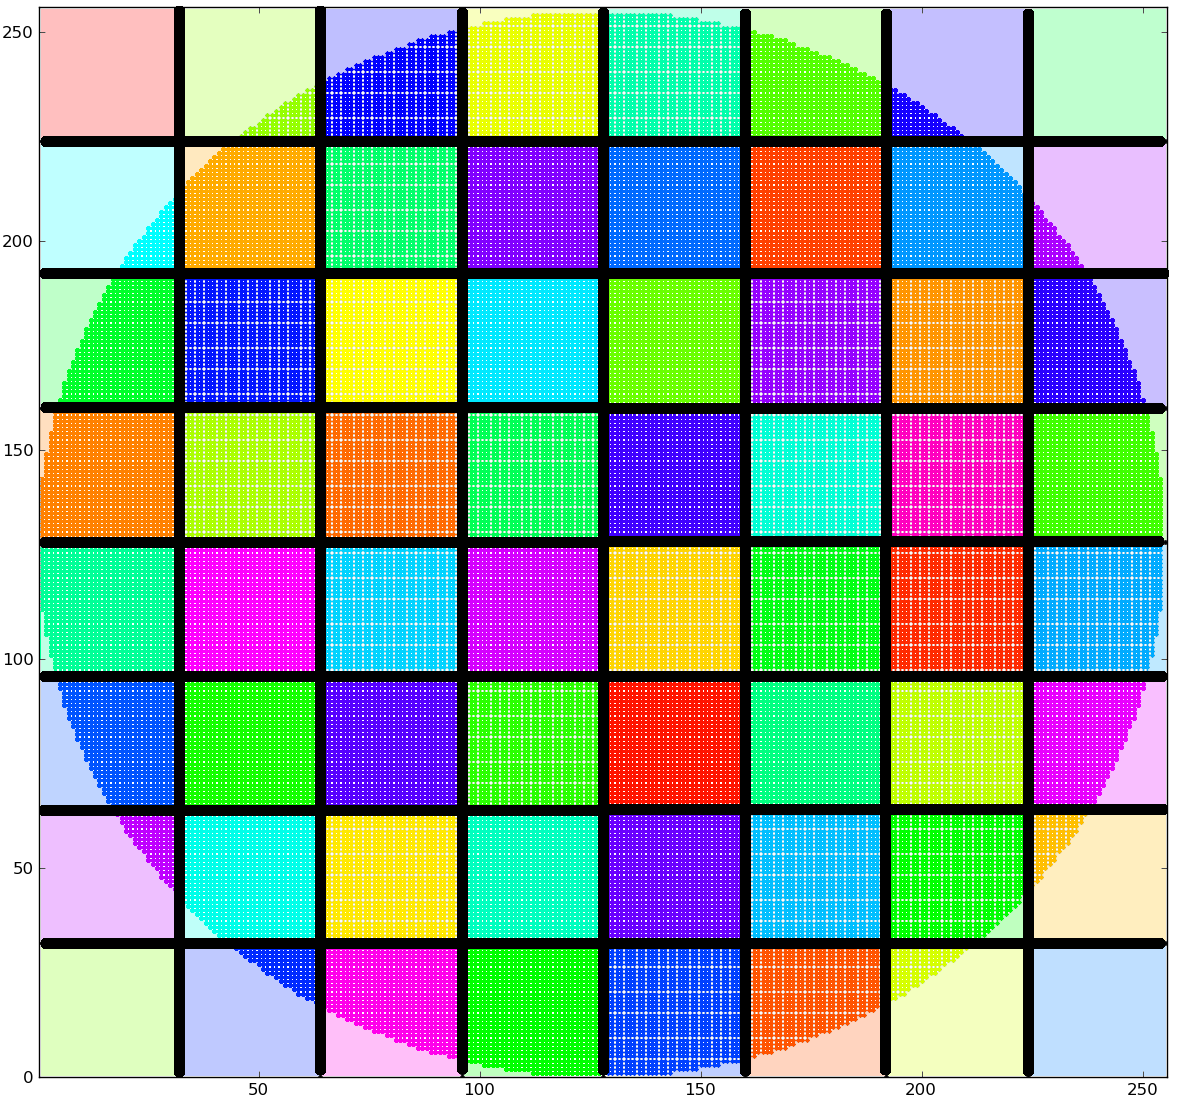
\includegraphics[width=0.45\textwidth]{plots/dist_1_rect.png}
  \hspace*{0.04\textwidth}
  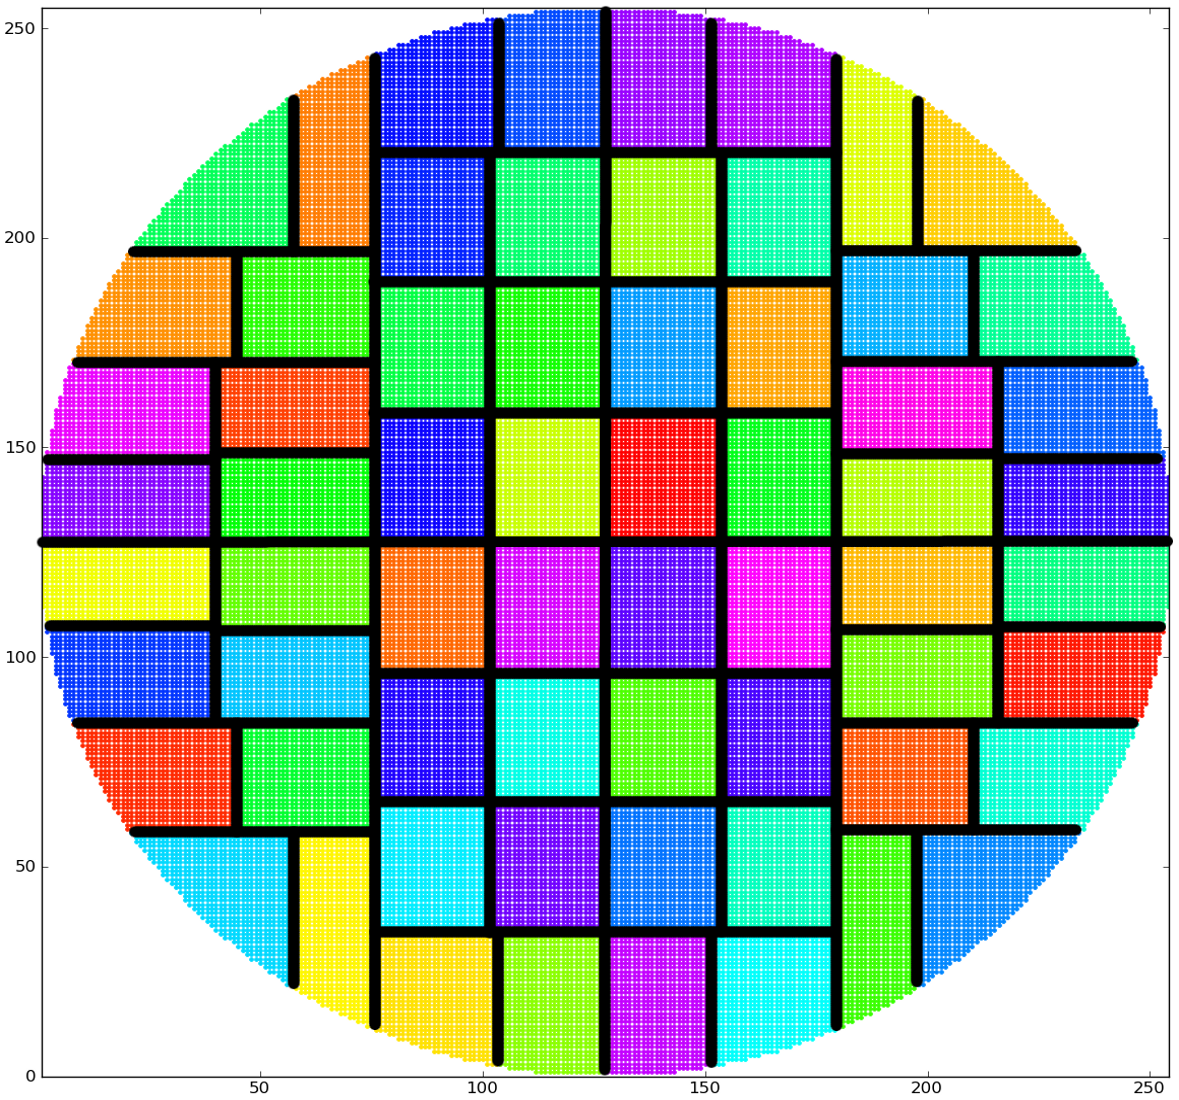
\includegraphics[width=0.45\textwidth]{plots/dist_1.png}
  \caption{(\textsc{Left}) Cross section of data distribution on $512$
    cores on a $8\!\times\!8\!\times\!8$ processor grid~(colors indicate
    data owned by a processor) and (\textsc{Right}) the same data
    redistributed with recursive coordinate bisection (RCB).}
  \label{fig:domcomp}
\end{figure}
%%
In Fig.~\ref{fig:domcomp} on the left a cross section is shown of the
case where the computational domain is embedded in a cube that has been
subdivided in $8\!\times\!8\!\times\!8$ subcubes.  It is easily seen
that the four subcubes in the corners do not contain any points of the
computational grid, while other subcubes contain at least a few grid
points.  In general, a fraction of only about $\pi/4\approx0.8$ of the
grid points of the cube will be included in the computational domain.
This number corresponds to the ratio of the volumes of the circular
cylinder and its encasing cube.  That is, about 20\% of the nodes in the
cube are not involved in the computation and, hence about 20\% of the
subcubes contain a reduced number of nodes.  Since subcubes correspond
to cores, empty or almost empty subcubes correspond to idle or
underloaded cores.

Evidently, this partitioning entails a severe load imbalance.
Nevertheless, the speedups shown in
Table~\ref{tab:timings_solver_1024_origpart_klu} look good! 
%%
These good speedups are comprehensible if one considers the most loaded
processes that correspond to the innermost cubes, i.e., those close to
the $z$-axis.  These subcubes contain $1024^3/p$ nodes.  An increase of
the processor number $p$ leads to an optimal speedup, at least as long
as the floating point operations dominate the work load.  This is the
case here, as even in the 2048~processor computation a core handles more
than half a million nodes.

Although speedups are good with this crude distribution of work, a
better balanced work will lead to improved execution times.  After all,
there are only about 80\% of the 1.1~billion nodes inside the
computational domain.

To better balance the load we partition data using the recursive
coordinate bisection (RCB) algorithm as it is implemented in the Zoltan
toolkit~\cite{ZoltanOverviewArticle,ZoltanUsersGuideV3}.  The Trilinos
package Isorropia%
\footnote{See \url{http://trilinos.sandia.gov/packages/isorropia/}}
provides a matrix-based interface to Zoltan.
%%
The recursive coordinate bisection (RCB) algorithm partitions the graph
according to the coordinates of its vertices.  The computational domain
is first divided into two subdomains by a cutting plane orthogonal to
one of the coordinate axes so that half the work load is in each of the
subdomains.  (Notice that other fractions than 50-50 are possible and in
fact needed if the number of processors is not a power of~2.)  That
coordinate axis is chosen which is associated with the longest
elongation of the domain.  Clearly, this procedure can be applied
recursively.  RCB leads to nicely balanced data distributions.
% in particular, if the computational domain is arranged along
% coordinate axes as in our case.
In rectangular grids, RCB is a particularly fast partitioner since the
coordinates of the grid vertices are easily determined from their
indices.
%%
In Fig.~\ref{fig:domcomp} on the right the cross section of the circular
cylinder is shown with the partitioning into 64~subdomains.  Now, all
subdomains contain an almost equal number of nodes which leads to almost
equal loads per processor.  This subdivision evidently is more
complicated than the one on the left of this figure.  Except for
subdomains in the center, i.e.\ close to the $z$ axis, there are more
than just six neighbors (in 3D).  With the increased number of neighbors
the number of messages that are to be sent in the communication steps
increases.  The communication volume does not change much.  (Notice that
Trilinos constructs the communication pattern transparent to the user.)
%%
\begin{table}[htb]
  \begin{center}
    \begin{tabular}{p{1cm}*{4}{p{20mm}}c}
      \hline
      cores & 
      solution & 
      construction & 
      application & 
      total ML & 
      iterations\\
      \hline
      512  & 50.32 [1.00] & 27.37 [1.00] & 44.00 [1.00] & 71.37 [1.00] & 20 \\
      1024 & 28.14 [0.89] & 16.82 [0.81] & 24.82 [0.89] & 41.58 [0.86] & 20 \\
      2048 & 15.26 [0.82] & 15.81 [0.43] & 13.47 [0.82] & 29.28 [0.61] & 19 \\
      \hline\\[-1mm]
    \end{tabular}
    \caption{Times in seconds and relative parallel efficiencies.  Data
      is distributed by RCB.  The coarsest AMG level is solved with
      KLU.%
      \vspace*{-10mm}
    }
    \label{tab:timings_solver_1024_rcb_klu}
  \end{center}
\end{table}
%%
\begin{table}[htb]
  \begin{center}
    \begin{tabular}{p{1cm}*{4}{p{20mm}}c}
      \hline
      cores & 
      solution & 
      construction & 
      application & 
      total ML & 
      iterations\\
      \hline
      512  & 51.08 [1.00] & 25.65 [1.00] & 44.89 [1.00] & 70.55 [1.00] & 20 \\
      1024 & 27.38 [0.93] & 12.96 [0.99] & 24.51 [0.92] & 37.07 [0.95] & 20 \\
      2048 & 14.76 [0.87] &  6.69 [0.96] & 13.10 [0.86] & 19.79 [0.89] & 19 \\
      \hline\\[-1mm]
    \end{tabular}
    \caption{Times in seconds and relative parallel efficiencies.  Data
      is distributed by RCB.  The coarsest AMG level is solved
      iteratively.%
      \vspace*{-5mm}%
    }
    \label{tab:timings_solver_1024_rcb_cheb}
  \end{center}
\end{table}

In Tables~\ref{tab:timings_solver_1024_rcb_klu}
and~\ref{tab:timings_solver_1024_rcb_cheb} the execution times of our
code is given with the data redistributed by RCB.  These numbers are to
be compared with those in
Tables~\ref{tab:timings_solver_1024_origpart_klu}
and~\ref{tab:timings_solver_1024_origpart_cheb}, respectively, where the
original data distribution was used.  For 512 cores the execution times
are significantly smaller with the RCB distribution, about 20\%, as the
previous discussion suggests.
%%
\begin{table}[tb]
  \begin{center}
    \begin{tabular}{p{1cm}*{4}{p{20mm}}}
      \hline
      cores & 
      solution & 
      construction & 
      application & 
      total ML \\
      \hline
      512  & 1.00 [0.81] & 1.00 [0.78] & 1.00 [0.85] & 1.00 [0.82] \\
      1024 & 0.89 [0.76] & 0.81 [0.69] & 0.89 [0.80] & 0.86 [0.75] \\
      2048 & 0.82 [0.71] & 0.43 [0.55] & 0.82 [0.74] & 0.61 [0.66] \\
      \hline\\[-1mm]
    \end{tabular}
    \caption{Parallel efficiencies of the RCB partitioned runs and
      relative parallel efficiencies of the runs with original data
      distribution.  The coarsest AMG level is solved with KLU.%
    }
    \label{tab:eff_solver_1024_rcb_klu}
  \end{center}
\end{table}
%%
\begin{table}
  \begin{center}
    \begin{tabular}{p{1cm}*{4}{p{20mm}}}
      \hline
      cores & 
      solution & 
      construction & 
      application & 
      total ML \\
      \hline
      512  & 1.00 [0.81] & 1.00 [0.80] & 1.00 [0.85] & 1.00 [0.83] \\
      1024 & 0.93 [0.76] & 0.99 [0.79] & 0.92 [0.80] & 0.95 [0.80] \\
      2048 & 0.87 [0.69] & 0.96 [0.79] & 0.86 [0.72] & 0.89 [0.74] \\
      \hline\\[-1mm]
    \end{tabular}
    \caption{Parallel efficiencies of the RCB partitioned runs and
      relative parallel efficiencies of the runs with original data
      distribution. The coarsest AMG level is solved iteratively.%
    }
    \label{tab:eff_solver_1024_rcb_cheb}
  \end{center}
\end{table}
%%
Tables~\ref{tab:eff_solver_1024_rcb_klu}
and~\ref{tab:eff_solver_1024_rcb_cheb} give more details.  There, in
brackets, the efficiencies of the runs with the original rectangular
distribution are listed relative to the 512~processor run with the RCB
distribution.

When using the iterative solver on the coarsest level, speedups and thus
efficiencies are quite close,
cf.~Tables~\ref{tab:timings_solver_1024_origpart_cheb}
and~\ref{tab:timings_solver_1024_rcb_cheb}.
%%
However, there are significant differences when the coarsest level
system is solved directly.  In this case the efficiencies deteriorate
more quickly with the RCB distribution than with the original
distribution.
%
A more detailed analysis (not reproduced here) reveals that the
significant difference between original and RCB partitioning is caused
by the LU factorization of the matrix of the coarsest level.  In fact,
the factorization takes 3.64\,sec on 1024 cores and 7.86\,sec on 2048.
We do not see a reason for this drastic increase of factorization time
since the problem sizes are quite close (2048 vs.\ 1865).  The fact that
the partitions with RCB have more neighbors does not seem to be a strong
enough reason.  In any case, larger differences would have to be visible
in Tables~\ref{tab:timings_solver_1024_origpart_cheb}
\emph{and}~\ref{tab:timings_solver_1024_rcb_cheb}.

In this paper we restricted ourselves to problems posed on grids of size
$1024\times1024\times1024$.  In~\cite{adai:10}, investigating the
original solver, we als included $512\times512\times512$ and
$256\times256\times256$ grids.  On the former grid the solver scaled
similarly as on the $1024^3$ grid, on the latter grid quite poorly.  By
replacing the direct coarse level solver by an iterative coarse level
solver we expect similar improvements in the parallel performance of our
solver also for these smaller problem sizes.  

% Furthermore the slightly better balanced data distribution should
% not affect the scalability decisively since it seems to be bound mainly
% by the size of the coarse level problem.

\section{Conclusions}
\label{sec:concl}

We have presented and discussed improvements of a scalable Poisson
solver suitable to handle domains with irregular boundaries as they
arise, for example, in beam dynamics simulations.  The solver employs
the conjugate gradient algorithm preconditioned by smoothed
aggregation-based AMG.  The code exhibits excellent scalability up to
2048 processors with cylindrical pipes embedded in meshes with up to
$1024^3$ grid points.  We have reduced the execution time by about 20\%
by redistributing the data using the recursive coordinate bisection
(RCB) algorithm.  This removes the severe load imbalance of the original
approach in~\cite{adai:10}.  Scalability was further improved by
iteratively solving the linear system of equations on the coarsest level
of the AMG preconditioner.

\section*{Acknowledgment}

These computations have been performed in the framework of a Large User
Project grant of the Swiss National Supercomputing Centre (CSCS).  We
acknowledge the help of the Cray support team at CSCS.

\bibliographystyle{abbrv}
\bibliography{para10.bib}

\end{document}
